% Created by tikzDevice version 0.7.0 on 2014-06-22 21:46:54
% !TEX encoding = UTF-8 Unicode
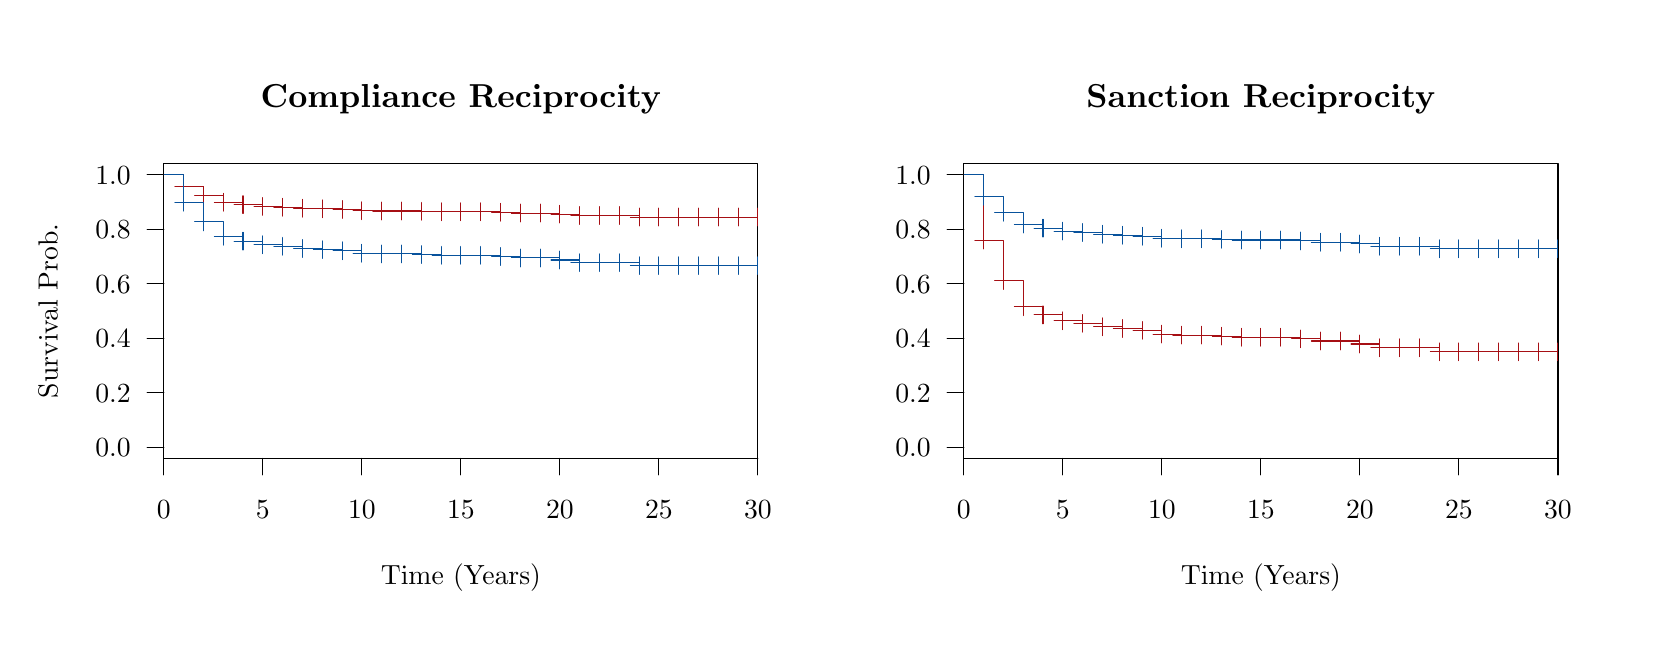
\begin{tikzpicture}[x=1pt,y=1pt]
\definecolor[named]{fillColor}{rgb}{1.00,1.00,1.00}
\path[use as bounding box,fill=fillColor,fill opacity=0.00] (0,0) rectangle (578.16,216.81);
\begin{scope}
\path[clip] (  0.00,  0.00) rectangle (578.16,216.81);
\definecolor[named]{drawColor}{rgb}{0.00,0.00,0.00}

\path[draw=drawColor,line width= 0.4pt,line join=round,line cap=round] ( 49.20, 61.20) -- (263.88, 61.20);

\path[draw=drawColor,line width= 0.4pt,line join=round,line cap=round] ( 49.20, 61.20) -- ( 49.20, 55.20);

\path[draw=drawColor,line width= 0.4pt,line join=round,line cap=round] ( 84.98, 61.20) -- ( 84.98, 55.20);

\path[draw=drawColor,line width= 0.4pt,line join=round,line cap=round] (120.76, 61.20) -- (120.76, 55.20);

\path[draw=drawColor,line width= 0.4pt,line join=round,line cap=round] (156.54, 61.20) -- (156.54, 55.20);

\path[draw=drawColor,line width= 0.4pt,line join=round,line cap=round] (192.32, 61.20) -- (192.32, 55.20);

\path[draw=drawColor,line width= 0.4pt,line join=round,line cap=round] (228.10, 61.20) -- (228.10, 55.20);

\path[draw=drawColor,line width= 0.4pt,line join=round,line cap=round] (263.88, 61.20) -- (263.88, 55.20);

\node[text=drawColor,anchor=base,inner sep=0pt, outer sep=0pt, scale=  1.00] at ( 49.20, 39.60) {0};

\node[text=drawColor,anchor=base,inner sep=0pt, outer sep=0pt, scale=  1.00] at ( 84.98, 39.60) {5};

\node[text=drawColor,anchor=base,inner sep=0pt, outer sep=0pt, scale=  1.00] at (120.76, 39.60) {10};

\node[text=drawColor,anchor=base,inner sep=0pt, outer sep=0pt, scale=  1.00] at (156.54, 39.60) {15};

\node[text=drawColor,anchor=base,inner sep=0pt, outer sep=0pt, scale=  1.00] at (192.32, 39.60) {20};

\node[text=drawColor,anchor=base,inner sep=0pt, outer sep=0pt, scale=  1.00] at (228.10, 39.60) {25};

\node[text=drawColor,anchor=base,inner sep=0pt, outer sep=0pt, scale=  1.00] at (263.88, 39.60) {30};

\path[draw=drawColor,line width= 0.4pt,line join=round,line cap=round] ( 49.20, 65.14) -- ( 49.20,163.67);

\path[draw=drawColor,line width= 0.4pt,line join=round,line cap=round] ( 49.20, 65.14) -- ( 43.20, 65.14);

\path[draw=drawColor,line width= 0.4pt,line join=round,line cap=round] ( 49.20, 84.85) -- ( 43.20, 84.85);

\path[draw=drawColor,line width= 0.4pt,line join=round,line cap=round] ( 49.20,104.55) -- ( 43.20,104.55);

\path[draw=drawColor,line width= 0.4pt,line join=round,line cap=round] ( 49.20,124.26) -- ( 43.20,124.26);

\path[draw=drawColor,line width= 0.4pt,line join=round,line cap=round] ( 49.20,143.96) -- ( 43.20,143.96);

\path[draw=drawColor,line width= 0.4pt,line join=round,line cap=round] ( 49.20,163.67) -- ( 43.20,163.67);

\node[text=drawColor,anchor=base east,inner sep=0pt, outer sep=0pt, scale=  1.00] at ( 37.20, 61.70) {0.0};

\node[text=drawColor,anchor=base east,inner sep=0pt, outer sep=0pt, scale=  1.00] at ( 37.20, 81.40) {0.2};

\node[text=drawColor,anchor=base east,inner sep=0pt, outer sep=0pt, scale=  1.00] at ( 37.20,101.11) {0.4};

\node[text=drawColor,anchor=base east,inner sep=0pt, outer sep=0pt, scale=  1.00] at ( 37.20,120.81) {0.6};

\node[text=drawColor,anchor=base east,inner sep=0pt, outer sep=0pt, scale=  1.00] at ( 37.20,140.52) {0.8};

\node[text=drawColor,anchor=base east,inner sep=0pt, outer sep=0pt, scale=  1.00] at ( 37.20,160.23) {1.0};

\path[draw=drawColor,line width= 0.4pt,line join=round,line cap=round] ( 49.20, 61.20) --
	(263.88, 61.20) --
	(263.88,167.61) --
	( 49.20,167.61) --
	( 49.20, 61.20);
\end{scope}
\begin{scope}
\path[clip] (  0.00,  0.00) rectangle (289.08,216.81);
\definecolor[named]{drawColor}{rgb}{0.00,0.00,0.00}

\node[text=drawColor,anchor=base,inner sep=0pt, outer sep=0pt, scale=  1.20] at (156.54,188.07) {\bfseries Compliance Reciprocity};
\end{scope}
\begin{scope}
\path[clip] ( 49.20, 61.20) rectangle (263.88,167.61);
\definecolor[named]{drawColor}{rgb}{0.65,0.06,0.08}

\path[draw=drawColor,line width= 0.4pt,line join=round,line cap=round] ( 49.20,163.67) --
	( 56.36,163.67) --
	( 56.36,159.42) --
	( 63.51,159.42) --
	( 63.51,156.18) --
	( 70.67,156.18) --
	( 70.67,153.72) --
	( 77.82,153.72) --
	( 77.82,152.87) --
	( 84.98,152.87) --
	( 84.98,152.22) --
	( 92.14,152.22) --
	( 92.14,151.94) --
	( 99.29,151.94) --
	( 99.29,151.55) --
	(106.45,151.55) --
	(106.45,151.35) --
	(113.60,151.35) --
	(113.60,151.13) --
	(120.76,151.13) --
	(120.76,150.68) --
	(127.92,150.68) --
	(127.92,150.56) --
	(142.23,150.56) --
	(142.23,150.44) --
	(149.38,150.44) --
	(149.38,150.30) --
	(170.85,150.30) --
	(170.85,150.10) --
	(178.01,150.10) --
	(178.01,149.82) --
	(192.32,149.82) --
	(192.32,149.43) --
	(199.48,149.43) --
	(199.48,148.94) --
	(220.94,148.94) --
	(220.94,148.37) --
	(492.87,148.37) --
	(492.87,148.37);

\path[draw=drawColor,line width= 0.4pt,line join=round,line cap=round] ( 53.17,159.42) -- ( 59.54,159.42);

\path[draw=drawColor,line width= 0.4pt,line join=round,line cap=round] ( 56.36,156.23) -- ( 56.36,162.60);

\path[draw=drawColor,line width= 0.4pt,line join=round,line cap=round] ( 60.33,156.18) -- ( 66.69,156.18);

\path[draw=drawColor,line width= 0.4pt,line join=round,line cap=round] ( 63.51,153.00) -- ( 63.51,159.36);

\path[draw=drawColor,line width= 0.4pt,line join=round,line cap=round] ( 67.49,153.72) -- ( 73.85,153.72);

\path[draw=drawColor,line width= 0.4pt,line join=round,line cap=round] ( 70.67,150.54) -- ( 70.67,156.91);

\path[draw=drawColor,line width= 0.4pt,line join=round,line cap=round] ( 74.64,152.87) -- ( 81.01,152.87);

\path[draw=drawColor,line width= 0.4pt,line join=round,line cap=round] ( 77.82,149.69) -- ( 77.82,156.05);

\path[draw=drawColor,line width= 0.4pt,line join=round,line cap=round] ( 81.80,152.22) -- ( 88.16,152.22);

\path[draw=drawColor,line width= 0.4pt,line join=round,line cap=round] ( 84.98,149.04) -- ( 84.98,155.41);

\path[draw=drawColor,line width= 0.4pt,line join=round,line cap=round] ( 88.95,151.94) -- ( 95.32,151.94);

\path[draw=drawColor,line width= 0.4pt,line join=round,line cap=round] ( 92.14,148.76) -- ( 92.14,155.12);

\path[draw=drawColor,line width= 0.4pt,line join=round,line cap=round] ( 96.11,151.55) -- (102.47,151.55);

\path[draw=drawColor,line width= 0.4pt,line join=round,line cap=round] ( 99.29,148.37) -- ( 99.29,154.73);

\path[draw=drawColor,line width= 0.4pt,line join=round,line cap=round] (103.27,151.35) -- (109.63,151.35);

\path[draw=drawColor,line width= 0.4pt,line join=round,line cap=round] (106.45,148.16) -- (106.45,154.53);

\path[draw=drawColor,line width= 0.4pt,line join=round,line cap=round] (110.42,151.13) -- (116.79,151.13);

\path[draw=drawColor,line width= 0.4pt,line join=round,line cap=round] (113.60,147.95) -- (113.60,154.31);

\path[draw=drawColor,line width= 0.4pt,line join=round,line cap=round] (117.58,150.68) -- (123.94,150.68);

\path[draw=drawColor,line width= 0.4pt,line join=round,line cap=round] (120.76,147.50) -- (120.76,153.87);

\path[draw=drawColor,line width= 0.4pt,line join=round,line cap=round] (124.73,150.56) -- (131.10,150.56);

\path[draw=drawColor,line width= 0.4pt,line join=round,line cap=round] (127.92,147.38) -- (127.92,153.75);

\path[draw=drawColor,line width= 0.4pt,line join=round,line cap=round] (131.89,150.56) -- (138.25,150.56);

\path[draw=drawColor,line width= 0.4pt,line join=round,line cap=round] (135.07,147.38) -- (135.07,153.75);

\path[draw=drawColor,line width= 0.4pt,line join=round,line cap=round] (139.05,150.44) -- (145.41,150.44);

\path[draw=drawColor,line width= 0.4pt,line join=round,line cap=round] (142.23,147.26) -- (142.23,153.62);

\path[draw=drawColor,line width= 0.4pt,line join=round,line cap=round] (146.20,150.30) -- (152.57,150.30);

\path[draw=drawColor,line width= 0.4pt,line join=round,line cap=round] (149.38,147.12) -- (149.38,153.48);

\path[draw=drawColor,line width= 0.4pt,line join=round,line cap=round] (153.36,150.30) -- (159.72,150.30);

\path[draw=drawColor,line width= 0.4pt,line join=round,line cap=round] (156.54,147.12) -- (156.54,153.48);

\path[draw=drawColor,line width= 0.4pt,line join=round,line cap=round] (160.51,150.30) -- (166.88,150.30);

\path[draw=drawColor,line width= 0.4pt,line join=round,line cap=round] (163.70,147.12) -- (163.70,153.48);

\path[draw=drawColor,line width= 0.4pt,line join=round,line cap=round] (167.67,150.10) -- (174.03,150.10);

\path[draw=drawColor,line width= 0.4pt,line join=round,line cap=round] (170.85,146.92) -- (170.85,153.28);

\path[draw=drawColor,line width= 0.4pt,line join=round,line cap=round] (174.83,149.82) -- (181.19,149.82);

\path[draw=drawColor,line width= 0.4pt,line join=round,line cap=round] (178.01,146.64) -- (178.01,153.00);

\path[draw=drawColor,line width= 0.4pt,line join=round,line cap=round] (181.98,149.82) -- (188.35,149.82);

\path[draw=drawColor,line width= 0.4pt,line join=round,line cap=round] (185.16,146.64) -- (185.16,153.00);

\path[draw=drawColor,line width= 0.4pt,line join=round,line cap=round] (189.14,149.43) -- (195.50,149.43);

\path[draw=drawColor,line width= 0.4pt,line join=round,line cap=round] (192.32,146.25) -- (192.32,152.62);

\path[draw=drawColor,line width= 0.4pt,line join=round,line cap=round] (196.29,148.94) -- (202.66,148.94);

\path[draw=drawColor,line width= 0.4pt,line join=round,line cap=round] (199.48,145.76) -- (199.48,152.12);

\path[draw=drawColor,line width= 0.4pt,line join=round,line cap=round] (203.45,148.94) -- (209.81,148.94);

\path[draw=drawColor,line width= 0.4pt,line join=round,line cap=round] (206.63,145.76) -- (206.63,152.12);

\path[draw=drawColor,line width= 0.4pt,line join=round,line cap=round] (210.61,148.94) -- (216.97,148.94);

\path[draw=drawColor,line width= 0.4pt,line join=round,line cap=round] (213.79,145.76) -- (213.79,152.12);

\path[draw=drawColor,line width= 0.4pt,line join=round,line cap=round] (217.76,148.37) -- (224.13,148.37);

\path[draw=drawColor,line width= 0.4pt,line join=round,line cap=round] (220.94,145.19) -- (220.94,151.56);

\path[draw=drawColor,line width= 0.4pt,line join=round,line cap=round] (224.92,148.37) -- (231.28,148.37);

\path[draw=drawColor,line width= 0.4pt,line join=round,line cap=round] (228.10,145.19) -- (228.10,151.56);

\path[draw=drawColor,line width= 0.4pt,line join=round,line cap=round] (232.07,148.37) -- (238.44,148.37);

\path[draw=drawColor,line width= 0.4pt,line join=round,line cap=round] (235.26,145.19) -- (235.26,151.56);

\path[draw=drawColor,line width= 0.4pt,line join=round,line cap=round] (239.23,148.37) -- (245.59,148.37);

\path[draw=drawColor,line width= 0.4pt,line join=round,line cap=round] (242.41,145.19) -- (242.41,151.56);

\path[draw=drawColor,line width= 0.4pt,line join=round,line cap=round] (246.39,148.37) -- (252.75,148.37);

\path[draw=drawColor,line width= 0.4pt,line join=round,line cap=round] (249.57,145.19) -- (249.57,151.56);

\path[draw=drawColor,line width= 0.4pt,line join=round,line cap=round] (253.54,148.37) -- (259.91,148.37);

\path[draw=drawColor,line width= 0.4pt,line join=round,line cap=round] (256.72,145.19) -- (256.72,151.56);

\path[draw=drawColor,line width= 0.4pt,line join=round,line cap=round] (260.70,148.37) -- (267.06,148.37);

\path[draw=drawColor,line width= 0.4pt,line join=round,line cap=round] (263.88,145.19) -- (263.88,151.56);

\path[draw=drawColor,line width= 0.4pt,line join=round,line cap=round] (267.85,148.37) -- (274.22,148.37);

\path[draw=drawColor,line width= 0.4pt,line join=round,line cap=round] (271.04,145.19) -- (271.04,151.56);

\path[draw=drawColor,line width= 0.4pt,line join=round,line cap=round] (275.01,148.37) -- (281.37,148.37);

\path[draw=drawColor,line width= 0.4pt,line join=round,line cap=round] (278.19,145.19) -- (278.19,151.56);

\path[draw=drawColor,line width= 0.4pt,line join=round,line cap=round] (282.17,148.37) -- (288.53,148.37);

\path[draw=drawColor,line width= 0.4pt,line join=round,line cap=round] (285.35,145.19) -- (285.35,151.56);

\path[draw=drawColor,line width= 0.4pt,line join=round,line cap=round] (289.32,148.37) -- (295.69,148.37);

\path[draw=drawColor,line width= 0.4pt,line join=round,line cap=round] (292.50,145.19) -- (292.50,151.56);

\path[draw=drawColor,line width= 0.4pt,line join=round,line cap=round] (296.48,148.37) -- (302.84,148.37);

\path[draw=drawColor,line width= 0.4pt,line join=round,line cap=round] (299.66,145.19) -- (299.66,151.56);

\path[draw=drawColor,line width= 0.4pt,line join=round,line cap=round] (303.63,148.37) -- (310.00,148.37);

\path[draw=drawColor,line width= 0.4pt,line join=round,line cap=round] (306.82,145.19) -- (306.82,151.56);

\path[draw=drawColor,line width= 0.4pt,line join=round,line cap=round] (310.79,148.37) -- (317.15,148.37);

\path[draw=drawColor,line width= 0.4pt,line join=round,line cap=round] (313.97,145.19) -- (313.97,151.56);

\path[draw=drawColor,line width= 0.4pt,line join=round,line cap=round] (317.95,148.37) -- (324.31,148.37);

\path[draw=drawColor,line width= 0.4pt,line join=round,line cap=round] (321.13,145.19) -- (321.13,151.56);

\path[draw=drawColor,line width= 0.4pt,line join=round,line cap=round] (325.10,148.37) -- (331.47,148.37);

\path[draw=drawColor,line width= 0.4pt,line join=round,line cap=round] (328.28,145.19) -- (328.28,151.56);

\path[draw=drawColor,line width= 0.4pt,line join=round,line cap=round] (332.26,148.37) -- (338.62,148.37);

\path[draw=drawColor,line width= 0.4pt,line join=round,line cap=round] (335.44,145.19) -- (335.44,151.56);

\path[draw=drawColor,line width= 0.4pt,line join=round,line cap=round] (339.41,148.37) -- (345.78,148.37);

\path[draw=drawColor,line width= 0.4pt,line join=round,line cap=round] (342.60,145.19) -- (342.60,151.56);

\path[draw=drawColor,line width= 0.4pt,line join=round,line cap=round] (346.57,148.37) -- (352.93,148.37);

\path[draw=drawColor,line width= 0.4pt,line join=round,line cap=round] (349.75,145.19) -- (349.75,151.56);

\path[draw=drawColor,line width= 0.4pt,line join=round,line cap=round] (353.73,148.37) -- (360.09,148.37);

\path[draw=drawColor,line width= 0.4pt,line join=round,line cap=round] (356.91,145.19) -- (356.91,151.56);

\path[draw=drawColor,line width= 0.4pt,line join=round,line cap=round] (360.88,148.37) -- (367.25,148.37);

\path[draw=drawColor,line width= 0.4pt,line join=round,line cap=round] (364.06,145.19) -- (364.06,151.56);

\path[draw=drawColor,line width= 0.4pt,line join=round,line cap=round] (368.04,148.37) -- (374.40,148.37);

\path[draw=drawColor,line width= 0.4pt,line join=round,line cap=round] (371.22,145.19) -- (371.22,151.56);

\path[draw=drawColor,line width= 0.4pt,line join=round,line cap=round] (375.19,148.37) -- (381.56,148.37);

\path[draw=drawColor,line width= 0.4pt,line join=round,line cap=round] (378.38,145.19) -- (378.38,151.56);

\path[draw=drawColor,line width= 0.4pt,line join=round,line cap=round] (382.35,148.37) -- (388.71,148.37);

\path[draw=drawColor,line width= 0.4pt,line join=round,line cap=round] (385.53,145.19) -- (385.53,151.56);

\path[draw=drawColor,line width= 0.4pt,line join=round,line cap=round] (389.51,148.37) -- (395.87,148.37);

\path[draw=drawColor,line width= 0.4pt,line join=round,line cap=round] (392.69,145.19) -- (392.69,151.56);

\path[draw=drawColor,line width= 0.4pt,line join=round,line cap=round] (396.66,148.37) -- (403.03,148.37);

\path[draw=drawColor,line width= 0.4pt,line join=round,line cap=round] (399.84,145.19) -- (399.84,151.56);

\path[draw=drawColor,line width= 0.4pt,line join=round,line cap=round] (403.82,148.37) -- (410.18,148.37);

\path[draw=drawColor,line width= 0.4pt,line join=round,line cap=round] (407.00,145.19) -- (407.00,151.56);

\path[draw=drawColor,line width= 0.4pt,line join=round,line cap=round] (410.97,148.37) -- (417.34,148.37);

\path[draw=drawColor,line width= 0.4pt,line join=round,line cap=round] (414.16,145.19) -- (414.16,151.56);

\path[draw=drawColor,line width= 0.4pt,line join=round,line cap=round] (418.13,148.37) -- (424.49,148.37);

\path[draw=drawColor,line width= 0.4pt,line join=round,line cap=round] (421.31,145.19) -- (421.31,151.56);

\path[draw=drawColor,line width= 0.4pt,line join=round,line cap=round] (425.29,148.37) -- (431.65,148.37);

\path[draw=drawColor,line width= 0.4pt,line join=round,line cap=round] (428.47,145.19) -- (428.47,151.56);

\path[draw=drawColor,line width= 0.4pt,line join=round,line cap=round] (432.44,148.37) -- (438.81,148.37);

\path[draw=drawColor,line width= 0.4pt,line join=round,line cap=round] (435.62,145.19) -- (435.62,151.56);

\path[draw=drawColor,line width= 0.4pt,line join=round,line cap=round] (439.60,148.37) -- (445.96,148.37);

\path[draw=drawColor,line width= 0.4pt,line join=round,line cap=round] (442.78,145.19) -- (442.78,151.56);

\path[draw=drawColor,line width= 0.4pt,line join=round,line cap=round] (446.75,148.37) -- (453.12,148.37);

\path[draw=drawColor,line width= 0.4pt,line join=round,line cap=round] (449.94,145.19) -- (449.94,151.56);

\path[draw=drawColor,line width= 0.4pt,line join=round,line cap=round] (453.91,148.37) -- (460.27,148.37);

\path[draw=drawColor,line width= 0.4pt,line join=round,line cap=round] (457.09,145.19) -- (457.09,151.56);

\path[draw=drawColor,line width= 0.4pt,line join=round,line cap=round] (461.07,148.37) -- (467.43,148.37);

\path[draw=drawColor,line width= 0.4pt,line join=round,line cap=round] (464.25,145.19) -- (464.25,151.56);

\path[draw=drawColor,line width= 0.4pt,line join=round,line cap=round] (468.22,148.37) -- (474.59,148.37);

\path[draw=drawColor,line width= 0.4pt,line join=round,line cap=round] (471.40,145.19) -- (471.40,151.56);

\path[draw=drawColor,line width= 0.4pt,line join=round,line cap=round] (475.38,148.37) -- (481.74,148.37);

\path[draw=drawColor,line width= 0.4pt,line join=round,line cap=round] (478.56,145.19) -- (478.56,151.56);

\path[draw=drawColor,line width= 0.4pt,line join=round,line cap=round] (482.53,148.37) -- (488.90,148.37);

\path[draw=drawColor,line width= 0.4pt,line join=round,line cap=round] (485.72,145.19) -- (485.72,151.56);

\path[draw=drawColor,line width= 0.4pt,line join=round,line cap=round] (489.69,148.37) -- (496.05,148.37);

\path[draw=drawColor,line width= 0.4pt,line join=round,line cap=round] (492.87,145.19) -- (492.87,151.56);
\definecolor[named]{drawColor}{rgb}{0.03,0.32,0.61}

\path[draw=drawColor,line width= 0.4pt,line join=round,line cap=round] ( 49.20,163.67) --
	( 56.36,163.67) --
	( 56.36,153.76) --
	( 63.51,153.76) --
	( 63.51,146.62) --
	( 70.67,146.62) --
	( 70.67,141.43) --
	( 77.82,141.43) --
	( 77.82,139.67) --
	( 84.98,139.67) --
	( 84.98,138.37) --
	( 92.14,138.37) --
	( 92.14,137.79) --
	( 99.29,137.79) --
	( 99.29,137.01) --
	(106.45,137.01) --
	(106.45,136.60) --
	(113.60,136.60) --
	(113.60,136.18) --
	(120.76,136.18) --
	(120.76,135.29) --
	(127.92,135.29) --
	(127.92,135.06) --
	(142.23,135.06) --
	(142.23,134.81) --
	(149.38,134.81) --
	(149.38,134.53) --
	(170.85,134.53) --
	(170.85,134.14) --
	(178.01,134.14) --
	(178.01,133.60) --
	(192.32,133.60) --
	(192.32,132.85) --
	(199.48,132.85) --
	(199.48,131.90) --
	(220.94,131.90) --
	(220.94,130.83) --
	(492.87,130.83) --
	(492.87,130.83);

\path[draw=drawColor,line width= 0.4pt,line join=round,line cap=round] ( 53.17,153.76) -- ( 59.54,153.76);

\path[draw=drawColor,line width= 0.4pt,line join=round,line cap=round] ( 56.36,150.57) -- ( 56.36,156.94);

\path[draw=drawColor,line width= 0.4pt,line join=round,line cap=round] ( 60.33,146.62) -- ( 66.69,146.62);

\path[draw=drawColor,line width= 0.4pt,line join=round,line cap=round] ( 63.51,143.44) -- ( 63.51,149.80);

\path[draw=drawColor,line width= 0.4pt,line join=round,line cap=round] ( 67.49,141.43) -- ( 73.85,141.43);

\path[draw=drawColor,line width= 0.4pt,line join=round,line cap=round] ( 70.67,138.25) -- ( 70.67,144.61);

\path[draw=drawColor,line width= 0.4pt,line join=round,line cap=round] ( 74.64,139.67) -- ( 81.01,139.67);

\path[draw=drawColor,line width= 0.4pt,line join=round,line cap=round] ( 77.82,136.49) -- ( 77.82,142.85);

\path[draw=drawColor,line width= 0.4pt,line join=round,line cap=round] ( 81.80,138.37) -- ( 88.16,138.37);

\path[draw=drawColor,line width= 0.4pt,line join=round,line cap=round] ( 84.98,135.18) -- ( 84.98,141.55);

\path[draw=drawColor,line width= 0.4pt,line join=round,line cap=round] ( 88.95,137.79) -- ( 95.32,137.79);

\path[draw=drawColor,line width= 0.4pt,line join=round,line cap=round] ( 92.14,134.61) -- ( 92.14,140.97);

\path[draw=drawColor,line width= 0.4pt,line join=round,line cap=round] ( 96.11,137.01) -- (102.47,137.01);

\path[draw=drawColor,line width= 0.4pt,line join=round,line cap=round] ( 99.29,133.83) -- ( 99.29,140.19);

\path[draw=drawColor,line width= 0.4pt,line join=round,line cap=round] (103.27,136.60) -- (109.63,136.60);

\path[draw=drawColor,line width= 0.4pt,line join=round,line cap=round] (106.45,133.42) -- (106.45,139.78);

\path[draw=drawColor,line width= 0.4pt,line join=round,line cap=round] (110.42,136.18) -- (116.79,136.18);

\path[draw=drawColor,line width= 0.4pt,line join=round,line cap=round] (113.60,132.99) -- (113.60,139.36);

\path[draw=drawColor,line width= 0.4pt,line join=round,line cap=round] (117.58,135.29) -- (123.94,135.29);

\path[draw=drawColor,line width= 0.4pt,line join=round,line cap=round] (120.76,132.11) -- (120.76,138.48);

\path[draw=drawColor,line width= 0.4pt,line join=round,line cap=round] (124.73,135.06) -- (131.10,135.06);

\path[draw=drawColor,line width= 0.4pt,line join=round,line cap=round] (127.92,131.88) -- (127.92,138.24);

\path[draw=drawColor,line width= 0.4pt,line join=round,line cap=round] (131.89,135.06) -- (138.25,135.06);

\path[draw=drawColor,line width= 0.4pt,line join=round,line cap=round] (135.07,131.88) -- (135.07,138.24);

\path[draw=drawColor,line width= 0.4pt,line join=round,line cap=round] (139.05,134.81) -- (145.41,134.81);

\path[draw=drawColor,line width= 0.4pt,line join=round,line cap=round] (142.23,131.63) -- (142.23,137.99);

\path[draw=drawColor,line width= 0.4pt,line join=round,line cap=round] (146.20,134.53) -- (152.57,134.53);

\path[draw=drawColor,line width= 0.4pt,line join=round,line cap=round] (149.38,131.35) -- (149.38,137.72);

\path[draw=drawColor,line width= 0.4pt,line join=round,line cap=round] (153.36,134.53) -- (159.72,134.53);

\path[draw=drawColor,line width= 0.4pt,line join=round,line cap=round] (156.54,131.35) -- (156.54,137.72);

\path[draw=drawColor,line width= 0.4pt,line join=round,line cap=round] (160.51,134.53) -- (166.88,134.53);

\path[draw=drawColor,line width= 0.4pt,line join=round,line cap=round] (163.70,131.35) -- (163.70,137.72);

\path[draw=drawColor,line width= 0.4pt,line join=round,line cap=round] (167.67,134.14) -- (174.03,134.14);

\path[draw=drawColor,line width= 0.4pt,line join=round,line cap=round] (170.85,130.96) -- (170.85,137.32);

\path[draw=drawColor,line width= 0.4pt,line join=round,line cap=round] (174.83,133.60) -- (181.19,133.60);

\path[draw=drawColor,line width= 0.4pt,line join=round,line cap=round] (178.01,130.42) -- (178.01,136.78);

\path[draw=drawColor,line width= 0.4pt,line join=round,line cap=round] (181.98,133.60) -- (188.35,133.60);

\path[draw=drawColor,line width= 0.4pt,line join=round,line cap=round] (185.16,130.42) -- (185.16,136.78);

\path[draw=drawColor,line width= 0.4pt,line join=round,line cap=round] (189.14,132.85) -- (195.50,132.85);

\path[draw=drawColor,line width= 0.4pt,line join=round,line cap=round] (192.32,129.67) -- (192.32,136.04);

\path[draw=drawColor,line width= 0.4pt,line join=round,line cap=round] (196.29,131.90) -- (202.66,131.90);

\path[draw=drawColor,line width= 0.4pt,line join=round,line cap=round] (199.48,128.72) -- (199.48,135.08);

\path[draw=drawColor,line width= 0.4pt,line join=round,line cap=round] (203.45,131.90) -- (209.81,131.90);

\path[draw=drawColor,line width= 0.4pt,line join=round,line cap=round] (206.63,128.72) -- (206.63,135.08);

\path[draw=drawColor,line width= 0.4pt,line join=round,line cap=round] (210.61,131.90) -- (216.97,131.90);

\path[draw=drawColor,line width= 0.4pt,line join=round,line cap=round] (213.79,128.72) -- (213.79,135.08);

\path[draw=drawColor,line width= 0.4pt,line join=round,line cap=round] (217.76,130.83) -- (224.13,130.83);

\path[draw=drawColor,line width= 0.4pt,line join=round,line cap=round] (220.94,127.64) -- (220.94,134.01);

\path[draw=drawColor,line width= 0.4pt,line join=round,line cap=round] (224.92,130.83) -- (231.28,130.83);

\path[draw=drawColor,line width= 0.4pt,line join=round,line cap=round] (228.10,127.64) -- (228.10,134.01);

\path[draw=drawColor,line width= 0.4pt,line join=round,line cap=round] (232.07,130.83) -- (238.44,130.83);

\path[draw=drawColor,line width= 0.4pt,line join=round,line cap=round] (235.26,127.64) -- (235.26,134.01);

\path[draw=drawColor,line width= 0.4pt,line join=round,line cap=round] (239.23,130.83) -- (245.59,130.83);

\path[draw=drawColor,line width= 0.4pt,line join=round,line cap=round] (242.41,127.64) -- (242.41,134.01);

\path[draw=drawColor,line width= 0.4pt,line join=round,line cap=round] (246.39,130.83) -- (252.75,130.83);

\path[draw=drawColor,line width= 0.4pt,line join=round,line cap=round] (249.57,127.64) -- (249.57,134.01);

\path[draw=drawColor,line width= 0.4pt,line join=round,line cap=round] (253.54,130.83) -- (259.91,130.83);

\path[draw=drawColor,line width= 0.4pt,line join=round,line cap=round] (256.72,127.64) -- (256.72,134.01);

\path[draw=drawColor,line width= 0.4pt,line join=round,line cap=round] (260.70,130.83) -- (267.06,130.83);

\path[draw=drawColor,line width= 0.4pt,line join=round,line cap=round] (263.88,127.64) -- (263.88,134.01);

\path[draw=drawColor,line width= 0.4pt,line join=round,line cap=round] (267.85,130.83) -- (274.22,130.83);

\path[draw=drawColor,line width= 0.4pt,line join=round,line cap=round] (271.04,127.64) -- (271.04,134.01);

\path[draw=drawColor,line width= 0.4pt,line join=round,line cap=round] (275.01,130.83) -- (281.37,130.83);

\path[draw=drawColor,line width= 0.4pt,line join=round,line cap=round] (278.19,127.64) -- (278.19,134.01);

\path[draw=drawColor,line width= 0.4pt,line join=round,line cap=round] (282.17,130.83) -- (288.53,130.83);

\path[draw=drawColor,line width= 0.4pt,line join=round,line cap=round] (285.35,127.64) -- (285.35,134.01);

\path[draw=drawColor,line width= 0.4pt,line join=round,line cap=round] (289.32,130.83) -- (295.69,130.83);

\path[draw=drawColor,line width= 0.4pt,line join=round,line cap=round] (292.50,127.64) -- (292.50,134.01);

\path[draw=drawColor,line width= 0.4pt,line join=round,line cap=round] (296.48,130.83) -- (302.84,130.83);

\path[draw=drawColor,line width= 0.4pt,line join=round,line cap=round] (299.66,127.64) -- (299.66,134.01);

\path[draw=drawColor,line width= 0.4pt,line join=round,line cap=round] (303.63,130.83) -- (310.00,130.83);

\path[draw=drawColor,line width= 0.4pt,line join=round,line cap=round] (306.82,127.64) -- (306.82,134.01);

\path[draw=drawColor,line width= 0.4pt,line join=round,line cap=round] (310.79,130.83) -- (317.15,130.83);

\path[draw=drawColor,line width= 0.4pt,line join=round,line cap=round] (313.97,127.64) -- (313.97,134.01);

\path[draw=drawColor,line width= 0.4pt,line join=round,line cap=round] (317.95,130.83) -- (324.31,130.83);

\path[draw=drawColor,line width= 0.4pt,line join=round,line cap=round] (321.13,127.64) -- (321.13,134.01);

\path[draw=drawColor,line width= 0.4pt,line join=round,line cap=round] (325.10,130.83) -- (331.47,130.83);

\path[draw=drawColor,line width= 0.4pt,line join=round,line cap=round] (328.28,127.64) -- (328.28,134.01);

\path[draw=drawColor,line width= 0.4pt,line join=round,line cap=round] (332.26,130.83) -- (338.62,130.83);

\path[draw=drawColor,line width= 0.4pt,line join=round,line cap=round] (335.44,127.64) -- (335.44,134.01);

\path[draw=drawColor,line width= 0.4pt,line join=round,line cap=round] (339.41,130.83) -- (345.78,130.83);

\path[draw=drawColor,line width= 0.4pt,line join=round,line cap=round] (342.60,127.64) -- (342.60,134.01);

\path[draw=drawColor,line width= 0.4pt,line join=round,line cap=round] (346.57,130.83) -- (352.93,130.83);

\path[draw=drawColor,line width= 0.4pt,line join=round,line cap=round] (349.75,127.64) -- (349.75,134.01);

\path[draw=drawColor,line width= 0.4pt,line join=round,line cap=round] (353.73,130.83) -- (360.09,130.83);

\path[draw=drawColor,line width= 0.4pt,line join=round,line cap=round] (356.91,127.64) -- (356.91,134.01);

\path[draw=drawColor,line width= 0.4pt,line join=round,line cap=round] (360.88,130.83) -- (367.25,130.83);

\path[draw=drawColor,line width= 0.4pt,line join=round,line cap=round] (364.06,127.64) -- (364.06,134.01);

\path[draw=drawColor,line width= 0.4pt,line join=round,line cap=round] (368.04,130.83) -- (374.40,130.83);

\path[draw=drawColor,line width= 0.4pt,line join=round,line cap=round] (371.22,127.64) -- (371.22,134.01);

\path[draw=drawColor,line width= 0.4pt,line join=round,line cap=round] (375.19,130.83) -- (381.56,130.83);

\path[draw=drawColor,line width= 0.4pt,line join=round,line cap=round] (378.38,127.64) -- (378.38,134.01);

\path[draw=drawColor,line width= 0.4pt,line join=round,line cap=round] (382.35,130.83) -- (388.71,130.83);

\path[draw=drawColor,line width= 0.4pt,line join=round,line cap=round] (385.53,127.64) -- (385.53,134.01);

\path[draw=drawColor,line width= 0.4pt,line join=round,line cap=round] (389.51,130.83) -- (395.87,130.83);

\path[draw=drawColor,line width= 0.4pt,line join=round,line cap=round] (392.69,127.64) -- (392.69,134.01);

\path[draw=drawColor,line width= 0.4pt,line join=round,line cap=round] (396.66,130.83) -- (403.03,130.83);

\path[draw=drawColor,line width= 0.4pt,line join=round,line cap=round] (399.84,127.64) -- (399.84,134.01);

\path[draw=drawColor,line width= 0.4pt,line join=round,line cap=round] (403.82,130.83) -- (410.18,130.83);

\path[draw=drawColor,line width= 0.4pt,line join=round,line cap=round] (407.00,127.64) -- (407.00,134.01);

\path[draw=drawColor,line width= 0.4pt,line join=round,line cap=round] (410.97,130.83) -- (417.34,130.83);

\path[draw=drawColor,line width= 0.4pt,line join=round,line cap=round] (414.16,127.64) -- (414.16,134.01);

\path[draw=drawColor,line width= 0.4pt,line join=round,line cap=round] (418.13,130.83) -- (424.49,130.83);

\path[draw=drawColor,line width= 0.4pt,line join=round,line cap=round] (421.31,127.64) -- (421.31,134.01);

\path[draw=drawColor,line width= 0.4pt,line join=round,line cap=round] (425.29,130.83) -- (431.65,130.83);

\path[draw=drawColor,line width= 0.4pt,line join=round,line cap=round] (428.47,127.64) -- (428.47,134.01);

\path[draw=drawColor,line width= 0.4pt,line join=round,line cap=round] (432.44,130.83) -- (438.81,130.83);

\path[draw=drawColor,line width= 0.4pt,line join=round,line cap=round] (435.62,127.64) -- (435.62,134.01);

\path[draw=drawColor,line width= 0.4pt,line join=round,line cap=round] (439.60,130.83) -- (445.96,130.83);

\path[draw=drawColor,line width= 0.4pt,line join=round,line cap=round] (442.78,127.64) -- (442.78,134.01);

\path[draw=drawColor,line width= 0.4pt,line join=round,line cap=round] (446.75,130.83) -- (453.12,130.83);

\path[draw=drawColor,line width= 0.4pt,line join=round,line cap=round] (449.94,127.64) -- (449.94,134.01);

\path[draw=drawColor,line width= 0.4pt,line join=round,line cap=round] (453.91,130.83) -- (460.27,130.83);

\path[draw=drawColor,line width= 0.4pt,line join=round,line cap=round] (457.09,127.64) -- (457.09,134.01);

\path[draw=drawColor,line width= 0.4pt,line join=round,line cap=round] (461.07,130.83) -- (467.43,130.83);

\path[draw=drawColor,line width= 0.4pt,line join=round,line cap=round] (464.25,127.64) -- (464.25,134.01);

\path[draw=drawColor,line width= 0.4pt,line join=round,line cap=round] (468.22,130.83) -- (474.59,130.83);

\path[draw=drawColor,line width= 0.4pt,line join=round,line cap=round] (471.40,127.64) -- (471.40,134.01);

\path[draw=drawColor,line width= 0.4pt,line join=round,line cap=round] (475.38,130.83) -- (481.74,130.83);

\path[draw=drawColor,line width= 0.4pt,line join=round,line cap=round] (478.56,127.64) -- (478.56,134.01);

\path[draw=drawColor,line width= 0.4pt,line join=round,line cap=round] (482.53,130.83) -- (488.90,130.83);

\path[draw=drawColor,line width= 0.4pt,line join=round,line cap=round] (485.72,127.64) -- (485.72,134.01);

\path[draw=drawColor,line width= 0.4pt,line join=round,line cap=round] (489.69,130.83) -- (496.05,130.83);

\path[draw=drawColor,line width= 0.4pt,line join=round,line cap=round] (492.87,127.64) -- (492.87,134.01);
\end{scope}
\begin{scope}
\path[clip] (  0.00,  0.00) rectangle (289.08,216.81);
\definecolor[named]{drawColor}{rgb}{0.00,0.00,0.00}

\node[text=drawColor,rotate= 90.00,anchor=base,inner sep=0pt, outer sep=0pt, scale=  1.00] at ( 10.80,114.41) {Survival Prob.};

\node[text=drawColor,anchor=base,inner sep=0pt, outer sep=0pt, scale=  1.00] at (156.54, 15.60) {Time (Years)};
\end{scope}
\begin{scope}
\path[clip] (  0.00,  0.00) rectangle (578.16,216.81);
\definecolor[named]{drawColor}{rgb}{0.00,0.00,0.00}

\path[draw=drawColor,line width= 0.4pt,line join=round,line cap=round] (338.28, 61.20) -- (552.96, 61.20);

\path[draw=drawColor,line width= 0.4pt,line join=round,line cap=round] (338.28, 61.20) -- (338.28, 55.20);

\path[draw=drawColor,line width= 0.4pt,line join=round,line cap=round] (374.06, 61.20) -- (374.06, 55.20);

\path[draw=drawColor,line width= 0.4pt,line join=round,line cap=round] (409.84, 61.20) -- (409.84, 55.20);

\path[draw=drawColor,line width= 0.4pt,line join=round,line cap=round] (445.62, 61.20) -- (445.62, 55.20);

\path[draw=drawColor,line width= 0.4pt,line join=round,line cap=round] (481.40, 61.20) -- (481.40, 55.20);

\path[draw=drawColor,line width= 0.4pt,line join=round,line cap=round] (517.18, 61.20) -- (517.18, 55.20);

\path[draw=drawColor,line width= 0.4pt,line join=round,line cap=round] (552.96, 61.20) -- (552.96, 55.20);

\node[text=drawColor,anchor=base,inner sep=0pt, outer sep=0pt, scale=  1.00] at (338.28, 39.60) {0};

\node[text=drawColor,anchor=base,inner sep=0pt, outer sep=0pt, scale=  1.00] at (374.06, 39.60) {5};

\node[text=drawColor,anchor=base,inner sep=0pt, outer sep=0pt, scale=  1.00] at (409.84, 39.60) {10};

\node[text=drawColor,anchor=base,inner sep=0pt, outer sep=0pt, scale=  1.00] at (445.62, 39.60) {15};

\node[text=drawColor,anchor=base,inner sep=0pt, outer sep=0pt, scale=  1.00] at (481.40, 39.60) {20};

\node[text=drawColor,anchor=base,inner sep=0pt, outer sep=0pt, scale=  1.00] at (517.18, 39.60) {25};

\node[text=drawColor,anchor=base,inner sep=0pt, outer sep=0pt, scale=  1.00] at (552.96, 39.60) {30};

\path[draw=drawColor,line width= 0.4pt,line join=round,line cap=round] (338.28, 65.14) -- (338.28,163.67);

\path[draw=drawColor,line width= 0.4pt,line join=round,line cap=round] (338.28, 65.14) -- (332.28, 65.14);

\path[draw=drawColor,line width= 0.4pt,line join=round,line cap=round] (338.28, 84.85) -- (332.28, 84.85);

\path[draw=drawColor,line width= 0.4pt,line join=round,line cap=round] (338.28,104.55) -- (332.28,104.55);

\path[draw=drawColor,line width= 0.4pt,line join=round,line cap=round] (338.28,124.26) -- (332.28,124.26);

\path[draw=drawColor,line width= 0.4pt,line join=round,line cap=round] (338.28,143.96) -- (332.28,143.96);

\path[draw=drawColor,line width= 0.4pt,line join=round,line cap=round] (338.28,163.67) -- (332.28,163.67);

\node[text=drawColor,anchor=base east,inner sep=0pt, outer sep=0pt, scale=  1.00] at (326.28, 61.70) {0.0};

\node[text=drawColor,anchor=base east,inner sep=0pt, outer sep=0pt, scale=  1.00] at (326.28, 81.40) {0.2};

\node[text=drawColor,anchor=base east,inner sep=0pt, outer sep=0pt, scale=  1.00] at (326.28,101.11) {0.4};

\node[text=drawColor,anchor=base east,inner sep=0pt, outer sep=0pt, scale=  1.00] at (326.28,120.81) {0.6};

\node[text=drawColor,anchor=base east,inner sep=0pt, outer sep=0pt, scale=  1.00] at (326.28,140.52) {0.8};

\node[text=drawColor,anchor=base east,inner sep=0pt, outer sep=0pt, scale=  1.00] at (326.28,160.23) {1.0};

\path[draw=drawColor,line width= 0.4pt,line join=round,line cap=round] (338.28, 61.20) --
	(552.96, 61.20) --
	(552.96,167.61) --
	(338.28,167.61) --
	(338.28, 61.20);
\end{scope}
\begin{scope}
\path[clip] (289.08,  0.00) rectangle (578.16,216.81);
\definecolor[named]{drawColor}{rgb}{0.00,0.00,0.00}

\node[text=drawColor,anchor=base,inner sep=0pt, outer sep=0pt, scale=  1.20] at (445.62,188.07) {\bfseries Sanction Reciprocity};
\end{scope}
\begin{scope}
\path[clip] (338.28, 61.20) rectangle (552.96,167.61);
\definecolor[named]{drawColor}{rgb}{0.65,0.06,0.08}

\path[draw=drawColor,line width= 0.4pt,line join=round,line cap=round] (338.28,163.67) --
	(345.44,163.67) --
	(345.44,140.04) --
	(352.59,140.04) --
	(352.59,125.42) --
	(359.75,125.42) --
	(359.75,115.99) --
	(366.90,115.99) --
	(366.90,113.01) --
	(374.06,113.01) --
	(374.06,110.88) --
	(381.22,110.88) --
	(381.22,109.95) --
	(388.37,109.95) --
	(388.37,108.72) --
	(395.53,108.72) --
	(395.53,108.08) --
	(402.68,108.08) --
	(402.68,107.42) --
	(409.84,107.42) --
	(409.84,106.08) --
	(417.00,106.08) --
	(417.00,105.72) --
	(431.31,105.72) --
	(431.31,105.35) --
	(438.46,105.35) --
	(438.46,104.94) --
	(459.93,104.94) --
	(459.93,104.36) --
	(467.09,104.36) --
	(467.09,103.57) --
	(481.40,103.57) --
	(481.40,102.50) --
	(488.56,102.50) --
	(488.56,101.15) --
	(510.02,101.15) --
	(510.02, 99.67) --
	(578.16, 99.67);

\path[draw=drawColor,line width= 0.4pt,line join=round,line cap=round] (342.25,140.04) -- (348.62,140.04);

\path[draw=drawColor,line width= 0.4pt,line join=round,line cap=round] (345.44,136.86) -- (345.44,143.22);

\path[draw=drawColor,line width= 0.4pt,line join=round,line cap=round] (349.41,125.42) -- (355.77,125.42);

\path[draw=drawColor,line width= 0.4pt,line join=round,line cap=round] (352.59,122.24) -- (352.59,128.60);

\path[draw=drawColor,line width= 0.4pt,line join=round,line cap=round] (356.57,115.99) -- (362.93,115.99);

\path[draw=drawColor,line width= 0.4pt,line join=round,line cap=round] (359.75,112.81) -- (359.75,119.18);

\path[draw=drawColor,line width= 0.4pt,line join=round,line cap=round] (363.72,113.01) -- (370.09,113.01);

\path[draw=drawColor,line width= 0.4pt,line join=round,line cap=round] (366.90,109.83) -- (366.90,116.20);

\path[draw=drawColor,line width= 0.4pt,line join=round,line cap=round] (370.88,110.88) -- (377.24,110.88);

\path[draw=drawColor,line width= 0.4pt,line join=round,line cap=round] (374.06,107.69) -- (374.06,114.06);

\path[draw=drawColor,line width= 0.4pt,line join=round,line cap=round] (378.03,109.95) -- (384.40,109.95);

\path[draw=drawColor,line width= 0.4pt,line join=round,line cap=round] (381.22,106.77) -- (381.22,113.13);

\path[draw=drawColor,line width= 0.4pt,line join=round,line cap=round] (385.19,108.72) -- (391.55,108.72);

\path[draw=drawColor,line width= 0.4pt,line join=round,line cap=round] (388.37,105.54) -- (388.37,111.90);

\path[draw=drawColor,line width= 0.4pt,line join=round,line cap=round] (392.35,108.08) -- (398.71,108.08);

\path[draw=drawColor,line width= 0.4pt,line join=round,line cap=round] (395.53,104.90) -- (395.53,111.26);

\path[draw=drawColor,line width= 0.4pt,line join=round,line cap=round] (399.50,107.42) -- (405.87,107.42);

\path[draw=drawColor,line width= 0.4pt,line join=round,line cap=round] (402.68,104.24) -- (402.68,110.60);

\path[draw=drawColor,line width= 0.4pt,line join=round,line cap=round] (406.66,106.08) -- (413.02,106.08);

\path[draw=drawColor,line width= 0.4pt,line join=round,line cap=round] (409.84,102.89) -- (409.84,109.26);

\path[draw=drawColor,line width= 0.4pt,line join=round,line cap=round] (413.81,105.72) -- (420.18,105.72);

\path[draw=drawColor,line width= 0.4pt,line join=round,line cap=round] (417.00,102.54) -- (417.00,108.90);

\path[draw=drawColor,line width= 0.4pt,line join=round,line cap=round] (420.97,105.72) -- (427.33,105.72);

\path[draw=drawColor,line width= 0.4pt,line join=round,line cap=round] (424.15,102.54) -- (424.15,108.90);

\path[draw=drawColor,line width= 0.4pt,line join=round,line cap=round] (428.13,105.35) -- (434.49,105.35);

\path[draw=drawColor,line width= 0.4pt,line join=round,line cap=round] (431.31,102.17) -- (431.31,108.53);

\path[draw=drawColor,line width= 0.4pt,line join=round,line cap=round] (435.28,104.94) -- (441.65,104.94);

\path[draw=drawColor,line width= 0.4pt,line join=round,line cap=round] (438.46,101.76) -- (438.46,108.12);

\path[draw=drawColor,line width= 0.4pt,line join=round,line cap=round] (442.44,104.94) -- (448.80,104.94);

\path[draw=drawColor,line width= 0.4pt,line join=round,line cap=round] (445.62,101.76) -- (445.62,108.12);

\path[draw=drawColor,line width= 0.4pt,line join=round,line cap=round] (449.59,104.94) -- (455.96,104.94);

\path[draw=drawColor,line width= 0.4pt,line join=round,line cap=round] (452.78,101.76) -- (452.78,108.12);

\path[draw=drawColor,line width= 0.4pt,line join=round,line cap=round] (456.75,104.36) -- (463.11,104.36);

\path[draw=drawColor,line width= 0.4pt,line join=round,line cap=round] (459.93,101.18) -- (459.93,107.54);

\path[draw=drawColor,line width= 0.4pt,line join=round,line cap=round] (463.91,103.57) -- (470.27,103.57);

\path[draw=drawColor,line width= 0.4pt,line join=round,line cap=round] (467.09,100.39) -- (467.09,106.75);

\path[draw=drawColor,line width= 0.4pt,line join=round,line cap=round] (471.06,103.57) -- (477.43,103.57);

\path[draw=drawColor,line width= 0.4pt,line join=round,line cap=round] (474.24,100.39) -- (474.24,106.75);

\path[draw=drawColor,line width= 0.4pt,line join=round,line cap=round] (478.22,102.50) -- (484.58,102.50);

\path[draw=drawColor,line width= 0.4pt,line join=round,line cap=round] (481.40, 99.31) -- (481.40,105.68);

\path[draw=drawColor,line width= 0.4pt,line join=round,line cap=round] (485.37,101.15) -- (491.74,101.15);

\path[draw=drawColor,line width= 0.4pt,line join=round,line cap=round] (488.56, 97.97) -- (488.56,104.33);

\path[draw=drawColor,line width= 0.4pt,line join=round,line cap=round] (492.53,101.15) -- (498.89,101.15);

\path[draw=drawColor,line width= 0.4pt,line join=round,line cap=round] (495.71, 97.97) -- (495.71,104.33);

\path[draw=drawColor,line width= 0.4pt,line join=round,line cap=round] (499.69,101.15) -- (506.05,101.15);

\path[draw=drawColor,line width= 0.4pt,line join=round,line cap=round] (502.87, 97.97) -- (502.87,104.33);

\path[draw=drawColor,line width= 0.4pt,line join=round,line cap=round] (506.84, 99.67) -- (513.21, 99.67);

\path[draw=drawColor,line width= 0.4pt,line join=round,line cap=round] (510.02, 96.49) -- (510.02,102.85);

\path[draw=drawColor,line width= 0.4pt,line join=round,line cap=round] (514.00, 99.67) -- (520.36, 99.67);

\path[draw=drawColor,line width= 0.4pt,line join=round,line cap=round] (517.18, 96.49) -- (517.18,102.85);

\path[draw=drawColor,line width= 0.4pt,line join=round,line cap=round] (521.15, 99.67) -- (527.52, 99.67);

\path[draw=drawColor,line width= 0.4pt,line join=round,line cap=round] (524.34, 96.49) -- (524.34,102.85);

\path[draw=drawColor,line width= 0.4pt,line join=round,line cap=round] (528.31, 99.67) -- (534.67, 99.67);

\path[draw=drawColor,line width= 0.4pt,line join=round,line cap=round] (531.49, 96.49) -- (531.49,102.85);

\path[draw=drawColor,line width= 0.4pt,line join=round,line cap=round] (535.47, 99.67) -- (541.83, 99.67);

\path[draw=drawColor,line width= 0.4pt,line join=round,line cap=round] (538.65, 96.49) -- (538.65,102.85);

\path[draw=drawColor,line width= 0.4pt,line join=round,line cap=round] (542.62, 99.67) -- (548.99, 99.67);

\path[draw=drawColor,line width= 0.4pt,line join=round,line cap=round] (545.80, 96.49) -- (545.80,102.85);

\path[draw=drawColor,line width= 0.4pt,line join=round,line cap=round] (549.78, 99.67) -- (556.14, 99.67);

\path[draw=drawColor,line width= 0.4pt,line join=round,line cap=round] (552.96, 96.49) -- (552.96,102.85);

\path[draw=drawColor,line width= 0.4pt,line join=round,line cap=round] (556.93, 99.67) -- (563.30, 99.67);

\path[draw=drawColor,line width= 0.4pt,line join=round,line cap=round] (560.12, 96.49) -- (560.12,102.85);

\path[draw=drawColor,line width= 0.4pt,line join=round,line cap=round] (564.09, 99.67) -- (570.45, 99.67);

\path[draw=drawColor,line width= 0.4pt,line join=round,line cap=round] (567.27, 96.49) -- (567.27,102.85);

\path[draw=drawColor,line width= 0.4pt,line join=round,line cap=round] (571.25, 99.67) -- (577.61, 99.67);

\path[draw=drawColor,line width= 0.4pt,line join=round,line cap=round] (574.43, 96.49) -- (574.43,102.85);
\definecolor[named]{drawColor}{rgb}{0.03,0.32,0.61}

\path[draw=drawColor,line width= 0.4pt,line join=round,line cap=round] (338.28,163.67) --
	(345.44,163.67) --
	(345.44,155.84) --
	(352.59,155.84) --
	(352.59,150.09) --
	(359.75,150.09) --
	(359.75,145.84) --
	(366.90,145.84) --
	(366.90,144.38) --
	(374.06,144.38) --
	(374.06,143.29) --
	(381.22,143.29) --
	(381.22,142.81) --
	(388.37,142.81) --
	(388.37,142.16) --
	(395.53,142.16) --
	(395.53,141.82) --
	(402.68,141.82) --
	(402.68,141.46) --
	(409.84,141.46) --
	(409.84,140.72) --
	(417.00,140.72) --
	(417.00,140.52) --
	(431.31,140.52) --
	(431.31,140.31) --
	(438.46,140.31) --
	(438.46,140.08) --
	(459.93,140.08) --
	(459.93,139.75) --
	(467.09,139.75) --
	(467.09,139.29) --
	(481.40,139.29) --
	(481.40,138.66) --
	(488.56,138.66) --
	(488.56,137.85) --
	(510.02,137.85) --
	(510.02,136.94) --
	(578.16,136.94);

\path[draw=drawColor,line width= 0.4pt,line join=round,line cap=round] (342.25,155.84) -- (348.62,155.84);

\path[draw=drawColor,line width= 0.4pt,line join=round,line cap=round] (345.44,152.66) -- (345.44,159.02);

\path[draw=drawColor,line width= 0.4pt,line join=round,line cap=round] (349.41,150.09) -- (355.77,150.09);

\path[draw=drawColor,line width= 0.4pt,line join=round,line cap=round] (352.59,146.91) -- (352.59,153.27);

\path[draw=drawColor,line width= 0.4pt,line join=round,line cap=round] (356.57,145.84) -- (362.93,145.84);

\path[draw=drawColor,line width= 0.4pt,line join=round,line cap=round] (359.75,142.65) -- (359.75,149.02);

\path[draw=drawColor,line width= 0.4pt,line join=round,line cap=round] (363.72,144.38) -- (370.09,144.38);

\path[draw=drawColor,line width= 0.4pt,line join=round,line cap=round] (366.90,141.20) -- (366.90,147.56);

\path[draw=drawColor,line width= 0.4pt,line join=round,line cap=round] (370.88,143.29) -- (377.24,143.29);

\path[draw=drawColor,line width= 0.4pt,line join=round,line cap=round] (374.06,140.11) -- (374.06,146.48);

\path[draw=drawColor,line width= 0.4pt,line join=round,line cap=round] (378.03,142.81) -- (384.40,142.81);

\path[draw=drawColor,line width= 0.4pt,line join=round,line cap=round] (381.22,139.63) -- (381.22,145.99);

\path[draw=drawColor,line width= 0.4pt,line join=round,line cap=round] (385.19,142.16) -- (391.55,142.16);

\path[draw=drawColor,line width= 0.4pt,line join=round,line cap=round] (388.37,138.98) -- (388.37,145.34);

\path[draw=drawColor,line width= 0.4pt,line join=round,line cap=round] (392.35,141.82) -- (398.71,141.82);

\path[draw=drawColor,line width= 0.4pt,line join=round,line cap=round] (395.53,138.64) -- (395.53,145.00);

\path[draw=drawColor,line width= 0.4pt,line join=round,line cap=round] (399.50,141.46) -- (405.87,141.46);

\path[draw=drawColor,line width= 0.4pt,line join=round,line cap=round] (402.68,138.28) -- (402.68,144.64);

\path[draw=drawColor,line width= 0.4pt,line join=round,line cap=round] (406.66,140.72) -- (413.02,140.72);

\path[draw=drawColor,line width= 0.4pt,line join=round,line cap=round] (409.84,137.54) -- (409.84,143.90);

\path[draw=drawColor,line width= 0.4pt,line join=round,line cap=round] (413.81,140.52) -- (420.18,140.52);

\path[draw=drawColor,line width= 0.4pt,line join=round,line cap=round] (417.00,137.34) -- (417.00,143.70);

\path[draw=drawColor,line width= 0.4pt,line join=round,line cap=round] (420.97,140.52) -- (427.33,140.52);

\path[draw=drawColor,line width= 0.4pt,line join=round,line cap=round] (424.15,137.34) -- (424.15,143.70);

\path[draw=drawColor,line width= 0.4pt,line join=round,line cap=round] (428.13,140.31) -- (434.49,140.31);

\path[draw=drawColor,line width= 0.4pt,line join=round,line cap=round] (431.31,137.13) -- (431.31,143.49);

\path[draw=drawColor,line width= 0.4pt,line join=round,line cap=round] (435.28,140.08) -- (441.65,140.08);

\path[draw=drawColor,line width= 0.4pt,line join=round,line cap=round] (438.46,136.90) -- (438.46,143.26);

\path[draw=drawColor,line width= 0.4pt,line join=round,line cap=round] (442.44,140.08) -- (448.80,140.08);

\path[draw=drawColor,line width= 0.4pt,line join=round,line cap=round] (445.62,136.90) -- (445.62,143.26);

\path[draw=drawColor,line width= 0.4pt,line join=round,line cap=round] (449.59,140.08) -- (455.96,140.08);

\path[draw=drawColor,line width= 0.4pt,line join=round,line cap=round] (452.78,136.90) -- (452.78,143.26);

\path[draw=drawColor,line width= 0.4pt,line join=round,line cap=round] (456.75,139.75) -- (463.11,139.75);

\path[draw=drawColor,line width= 0.4pt,line join=round,line cap=round] (459.93,136.57) -- (459.93,142.93);

\path[draw=drawColor,line width= 0.4pt,line join=round,line cap=round] (463.91,139.29) -- (470.27,139.29);

\path[draw=drawColor,line width= 0.4pt,line join=round,line cap=round] (467.09,136.11) -- (467.09,142.48);

\path[draw=drawColor,line width= 0.4pt,line join=round,line cap=round] (471.06,139.29) -- (477.43,139.29);

\path[draw=drawColor,line width= 0.4pt,line join=round,line cap=round] (474.24,136.11) -- (474.24,142.48);

\path[draw=drawColor,line width= 0.4pt,line join=round,line cap=round] (478.22,138.66) -- (484.58,138.66);

\path[draw=drawColor,line width= 0.4pt,line join=round,line cap=round] (481.40,135.48) -- (481.40,141.84);

\path[draw=drawColor,line width= 0.4pt,line join=round,line cap=round] (485.37,137.85) -- (491.74,137.85);

\path[draw=drawColor,line width= 0.4pt,line join=round,line cap=round] (488.56,134.67) -- (488.56,141.03);

\path[draw=drawColor,line width= 0.4pt,line join=round,line cap=round] (492.53,137.85) -- (498.89,137.85);

\path[draw=drawColor,line width= 0.4pt,line join=round,line cap=round] (495.71,134.67) -- (495.71,141.03);

\path[draw=drawColor,line width= 0.4pt,line join=round,line cap=round] (499.69,137.85) -- (506.05,137.85);

\path[draw=drawColor,line width= 0.4pt,line join=round,line cap=round] (502.87,134.67) -- (502.87,141.03);

\path[draw=drawColor,line width= 0.4pt,line join=round,line cap=round] (506.84,136.94) -- (513.21,136.94);

\path[draw=drawColor,line width= 0.4pt,line join=round,line cap=round] (510.02,133.75) -- (510.02,140.12);

\path[draw=drawColor,line width= 0.4pt,line join=round,line cap=round] (514.00,136.94) -- (520.36,136.94);

\path[draw=drawColor,line width= 0.4pt,line join=round,line cap=round] (517.18,133.75) -- (517.18,140.12);

\path[draw=drawColor,line width= 0.4pt,line join=round,line cap=round] (521.15,136.94) -- (527.52,136.94);

\path[draw=drawColor,line width= 0.4pt,line join=round,line cap=round] (524.34,133.75) -- (524.34,140.12);

\path[draw=drawColor,line width= 0.4pt,line join=round,line cap=round] (528.31,136.94) -- (534.67,136.94);

\path[draw=drawColor,line width= 0.4pt,line join=round,line cap=round] (531.49,133.75) -- (531.49,140.12);

\path[draw=drawColor,line width= 0.4pt,line join=round,line cap=round] (535.47,136.94) -- (541.83,136.94);

\path[draw=drawColor,line width= 0.4pt,line join=round,line cap=round] (538.65,133.75) -- (538.65,140.12);

\path[draw=drawColor,line width= 0.4pt,line join=round,line cap=round] (542.62,136.94) -- (548.99,136.94);

\path[draw=drawColor,line width= 0.4pt,line join=round,line cap=round] (545.80,133.75) -- (545.80,140.12);

\path[draw=drawColor,line width= 0.4pt,line join=round,line cap=round] (549.78,136.94) -- (556.14,136.94);

\path[draw=drawColor,line width= 0.4pt,line join=round,line cap=round] (552.96,133.75) -- (552.96,140.12);

\path[draw=drawColor,line width= 0.4pt,line join=round,line cap=round] (556.93,136.94) -- (563.30,136.94);

\path[draw=drawColor,line width= 0.4pt,line join=round,line cap=round] (560.12,133.75) -- (560.12,140.12);

\path[draw=drawColor,line width= 0.4pt,line join=round,line cap=round] (564.09,136.94) -- (570.45,136.94);

\path[draw=drawColor,line width= 0.4pt,line join=round,line cap=round] (567.27,133.75) -- (567.27,140.12);

\path[draw=drawColor,line width= 0.4pt,line join=round,line cap=round] (571.25,136.94) -- (577.61,136.94);

\path[draw=drawColor,line width= 0.4pt,line join=round,line cap=round] (574.43,133.75) -- (574.43,140.12);
\end{scope}
\begin{scope}
\path[clip] (289.08,  0.00) rectangle (578.16,216.81);
\definecolor[named]{drawColor}{rgb}{0.00,0.00,0.00}

\node[text=drawColor,anchor=base,inner sep=0pt, outer sep=0pt, scale=  1.00] at (445.62, 15.60) {Time (Years)};
\end{scope}
\end{tikzpicture}
